
\documentclass[a4paper,14pt]{extreport}
\usepackage{cmap} % Улучшенный поиск русских слов в полученном pdf-файле
\usepackage[T2A]{fontenc} % Поддержка русских букв
\usepackage[utf8]{inputenc} % Кодировка utf8
\usepackage[english,russian]{babel} % Языки: русский, английский
%\usepackage{pscyr} % Нормальные шрифты
\usepackage{amsmath}
\usepackage{geometry}
\geometry{left=30mm}
\geometry{right=15mm}
\geometry{top=20mm}
\geometry{bottom=20mm}
\usepackage{titlesec}
%\usepackage[ruled,longend]{algorithm2e}
\usepackage{textgreek}
\usepackage{algpseudocode}
\usepackage{pgfplots}
\pgfplotsset{compat=1.9}
\usepackage{algorithm}
\renewcommand{\listalgorithmname}{Список алгоритмов}
\floatname{algorithm}{Алгоритм}
\usepackage{amssymb}
\titleformat{\section}
{\normalsize\bfseries}
{\thesection}
{1em}{}
\titlespacing*{\chapter}{0pt}{-30pt}{8pt}
\titlespacing*{\section}{\parindent}{*4}{*4}
\titlespacing*{\subsection}{\parindent}{*4}{*4}
\usepackage{setspace}
\usepackage{mathtools}
\usepackage{float}
\DeclarePairedDelimiter\bra{\langle}{\rvert}
\DeclarePairedDelimiter\ket{\lvert}{\rangle}
\DeclarePairedDelimiterX\braket[2]{\langle}{\rangle}{#1 \delimsize\vert #2}
\onehalfspacing % Полуторный интервал
\frenchspacing
\usepackage{indentfirst} % Красная строка
\usepackage{titlesec}
\titleformat{\chapter}{\LARGE\bfseries}{\thechapter}{20pt}{\LARGE\bfseries}
\titleformat{\section}{\Large\bfseries}{\thesection}{20pt}{\Large\bfseries}
\usepackage{listings}
\usepackage{xcolor}
\lstdefinestyle{rustlang}{
	language=Rust,
	backgroundcolor=\color{white},
	basicstyle=\footnotesize\ttfamily,
	keywordstyle=\color{purple},
	stringstyle=\color{green},
	commentstyle=\color{gray},
	numbers=left,
	stepnumber=1,
	numbersep=5pt,
	frame=single,
	tabsize=4,
	captionpos=t,
	breaklines=true,
	breakatwhitespace=true,
	escapeinside={\#*}{*)},
	morecomment=[l][\color{magenta}]{\#},
	columns=fullflexible
}
\usepackage{pgfplots}
\usetikzlibrary{datavisualization}
\usetikzlibrary{datavisualization.formats.functions}
\usepackage{graphicx}
\newcommand{\img}[3] {
	\begin{figure}[h]
		\center{\includegraphics[height=#1]{assets/img/#2}}
		\caption{#3}
		\label{img:#2}
	\end{figure}
}
\newcommand{\boximg}[3] {
	\begin{figure}[h]
		\center{\fbox{\includegraphics[height=#1]{assets/img/#2}}}
		\caption{#3}
		\label{img:#2}
	\end{figure}
}
\usepackage[justification=centering]{caption} % Настройка подписей float объектов
\usepackage[unicode,pdftex]{hyperref} % Ссылки в pdf
\hypersetup{hidelinks}
\newcommand{\code}[1]{\texttt{#1}}
\usepackage{icomma} % Интеллектуальные запятые для десятичных чисел
\usepackage{csvsimple}

\usepackage{color} %use color
\definecolor{mygreen}{rgb}{0,0.6,0}
\definecolor{mygray}{rgb}{0.5,0.5,0.5}
\definecolor{mymauve}{rgb}{0.58,0,0.82}



\definecolor{darkgray}{rgb}{.4,.4,.4}
\definecolor{purple}{rgb}{0.65, 0.12, 0.82}


\begin{document}
	%\def\chaptername{} % убирает "Глава"
	\thispagestyle{empty}
	\begin{titlepage}
		\noindent \begin{minipage}{0.15\textwidth}
			
\includegraphics[width=\linewidth]{img/b_logo}
		\end{minipage}
		\noindent\begin{minipage}{0.9\textwidth}\centering
			\textbf{Министерство науки и высшего образования Российской Федерации}\\
			\textbf{Федеральное государственное бюджетное образовательное учреждение высшего образования}\\
			\textbf{~~~«Московский государственный технический университет имени Н.Э.~Баумана}\\
			\textbf{(национальный исследовательский университет)»}\\
			\textbf{(МГТУ им. Н.Э.~Баумана)}
		\end{minipage}
		
		\noindent\rule{18cm}{3pt}
		\newline\newline
		\noindent ФАКУЛЬТЕТ $\underline{\text{«Информатика и системы управления»}}$ \newline\newline
		\noindent КАФЕДРА $\underline{\text{«Программное обеспечение ЭВМ и информационные технологии»}}$\newline\newline
		
		\begin{center}
			\noindent\begin{minipage}{1.1\textwidth}\centering
				\Large\textbf{  Отчет по лабораторной работе №6}\newline
				\textbf{по дисциплине <<Операционные системы>>}\newline
			\end{minipage}
		\end{center}
		
		\noindent\textbf{Тема} $\underline{\text{Системный вызов open()~~~~~}}$\newline\newline
		\noindent\textbf{Студент} $\underline{\text{Зайцева А. А.~~~~~~~~~~~~~}}$\newline\newline
		\noindent\textbf{Группа} $\underline{\text{ИУ7-62Б~~~~~~~~~~~~~~~~~~~~~}}$\newline\newline
		\noindent\textbf{Оценка (баллы)} $\underline{\text{~~~~~~~~~~~~~~~~~~~~}}$\newline\newline
		\noindent\textbf{Преподаватель} $\underline{\text{Рязанова Н. Ю.}}$\newline\newline\newline
		
		\begin{center}
			\vfill
			Москва~---~\the\year
			~г.
		\end{center}
	\end{titlepage}




\chapter{Схемы алгоритмов}

\section{open()}

\begin{figure}[H]
	\centering
	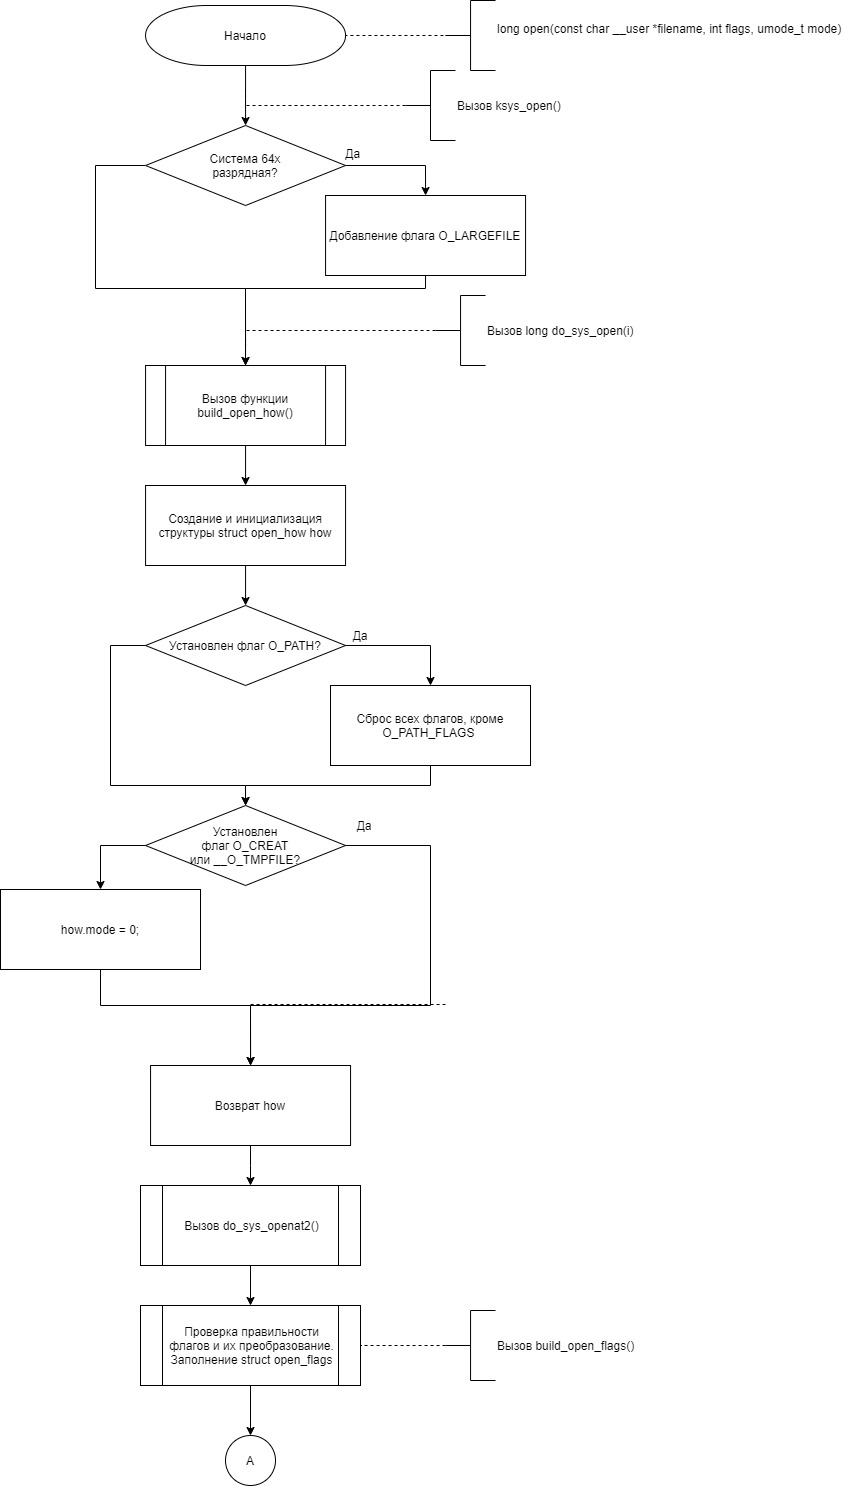
\includegraphics[scale=0.4]{img/open1.jpg}
\end{figure}





\section{$\texttt{build\_open\_how()}$}

\begin{lstlisting}[language=c, caption=Структура open_how и функция build_open_how()]
/*
 * Arguments for how openat2(2) should open the target path. If only @flags and
 * @mode are non-zero, then openat2(2) operates very similarly to openat(2).
 *
 * However, unlike openat(2), unknown or invalid bits in @flags result in
 * -EINVAL rather than being silently ignored. @mode must be zero unless one of
 * {O_CREAT, O_TMPFILE} are set.
 *
 * @flags: O_* flags.
 * @mode: O_CREAT/O_TMPFILE file mode.
 * @resolve: RESOLVE_* flags.
 */
struct open_how {
	__u64 flags;
	__u64 mode;
	__u64 resolve;
};


/* List of all valid flags for the open/openat flags argument: */
#define VALID_OPEN_FLAGS \
	(O_RDONLY | O_WRONLY | O_RDWR | O_CREAT | O_EXCL | O_NOCTTY | O_TRUNC | \
	 O_APPEND | O_NDELAY | O_NONBLOCK | __O_SYNC | O_DSYNC | \
	 FASYNC	| O_DIRECT | O_LARGEFILE | O_DIRECTORY | O_NOFOLLOW | \
	 O_NOATIME | O_CLOEXEC | O_PATH | __O_TMPFILE)
	 
#define S_IALLUGO	(S_ISUID|S_ISGID|S_ISVTX|S_IRWXUGO)

#define WILL_CREATE(flags)	(flags & (O_CREAT | __O_TMPFILE))
#define O_PATH_FLAGS		(O_DIRECTORY | O_NOFOLLOW | O_PATH | O_CLOEXEC)

inline struct open_how build_open_how(int flags, umode_t mode)
{
	struct open_how how = {
		.flags = flags & VALID_OPEN_FLAGS,
		.mode = mode & S_IALLUGO,
	};

	/* O_PATH beats everything else. */
	if (how.flags & O_PATH)
		how.flags &= O_PATH_FLAGS;
	/* Modes should only be set for create-like flags. */
	if (!WILL_CREATE(how.flags))
		how.mode = 0;
	return how;
}
\end{lstlisting}


\begin{figure}[H]
	\centering
	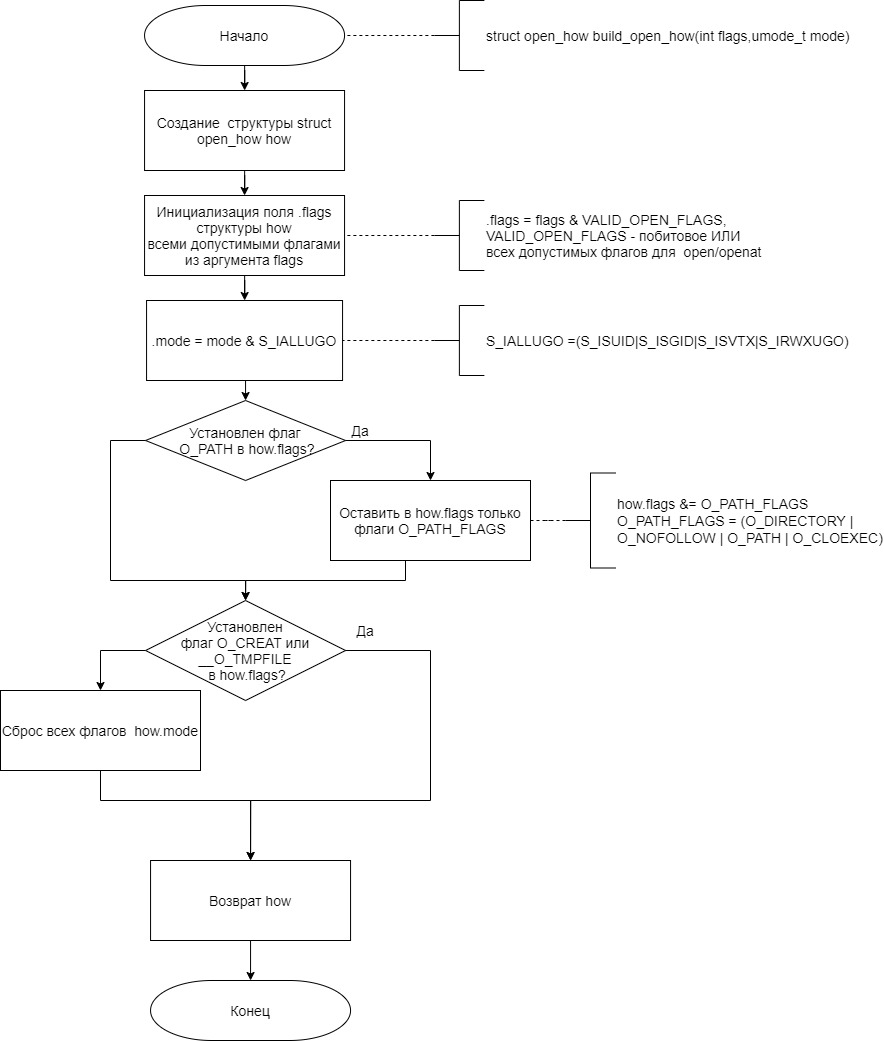
\includegraphics[scale=0.45]{img/build_open_how.jpg}
\end{figure}








\section{$\texttt{do\_sys\_openat2()}$}
\begin{figure}[H]
	\centering
	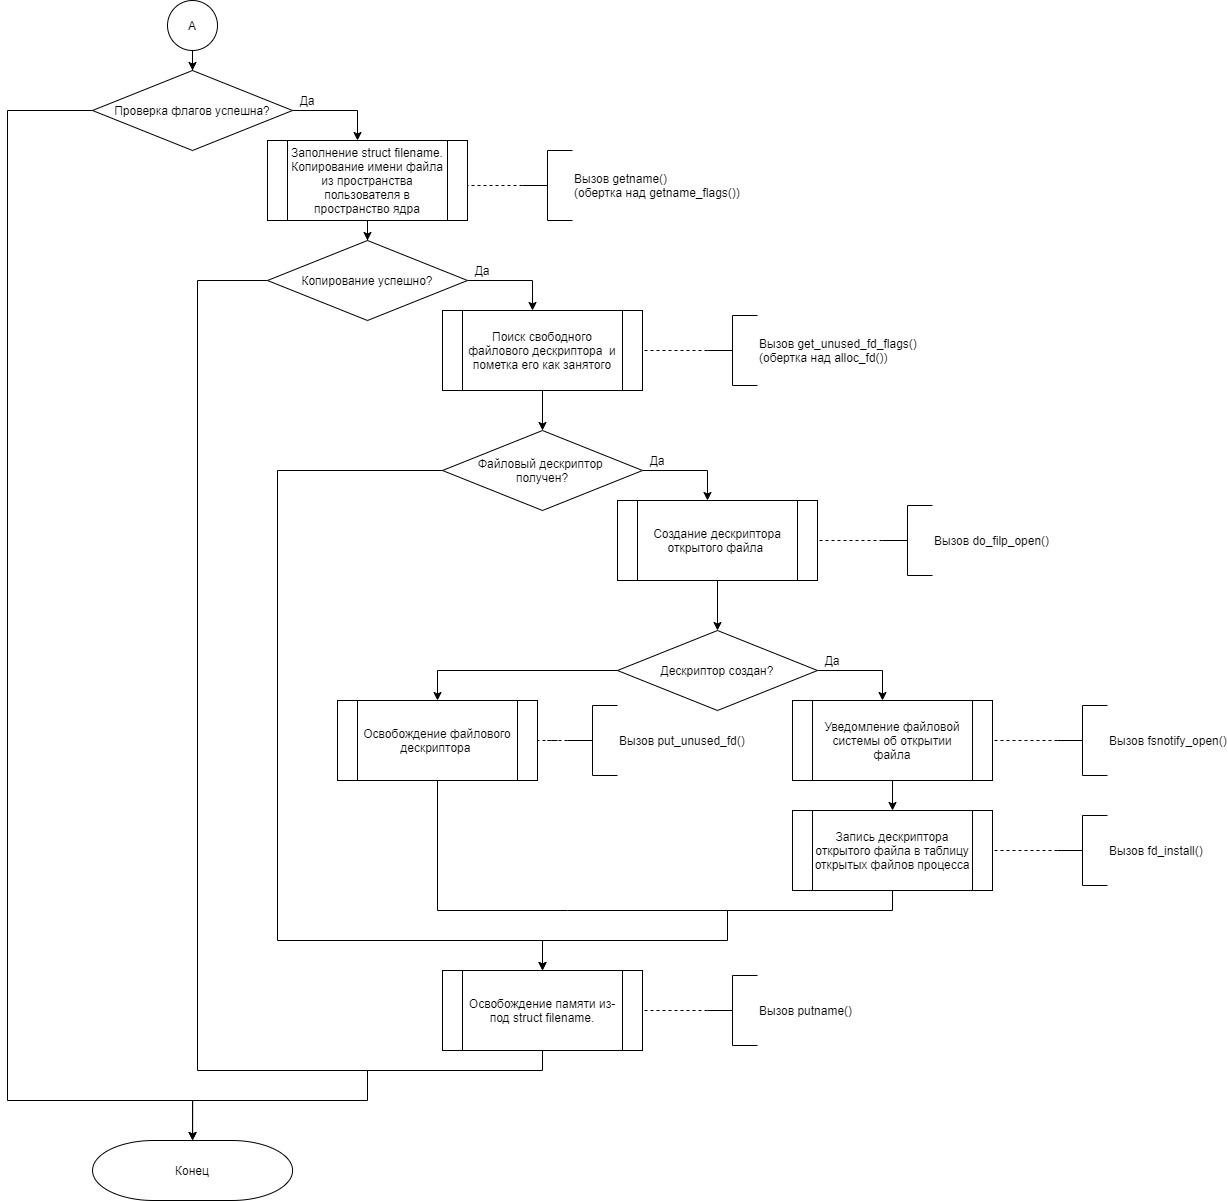
\includegraphics[scale=0.45]{img/open2.jpg}
\end{figure}










\section{$\texttt{build\_open\_flags()}$}

\begin{lstlisting}[language=c, caption=Структура open_flags]

struct open_flags {
	int open_flag;
	umode_t mode;
	int acc_mode;
	int intent;
	int lookup_flags;
};
\end{lstlisting}


\begin{figure}[H]
	\centering
	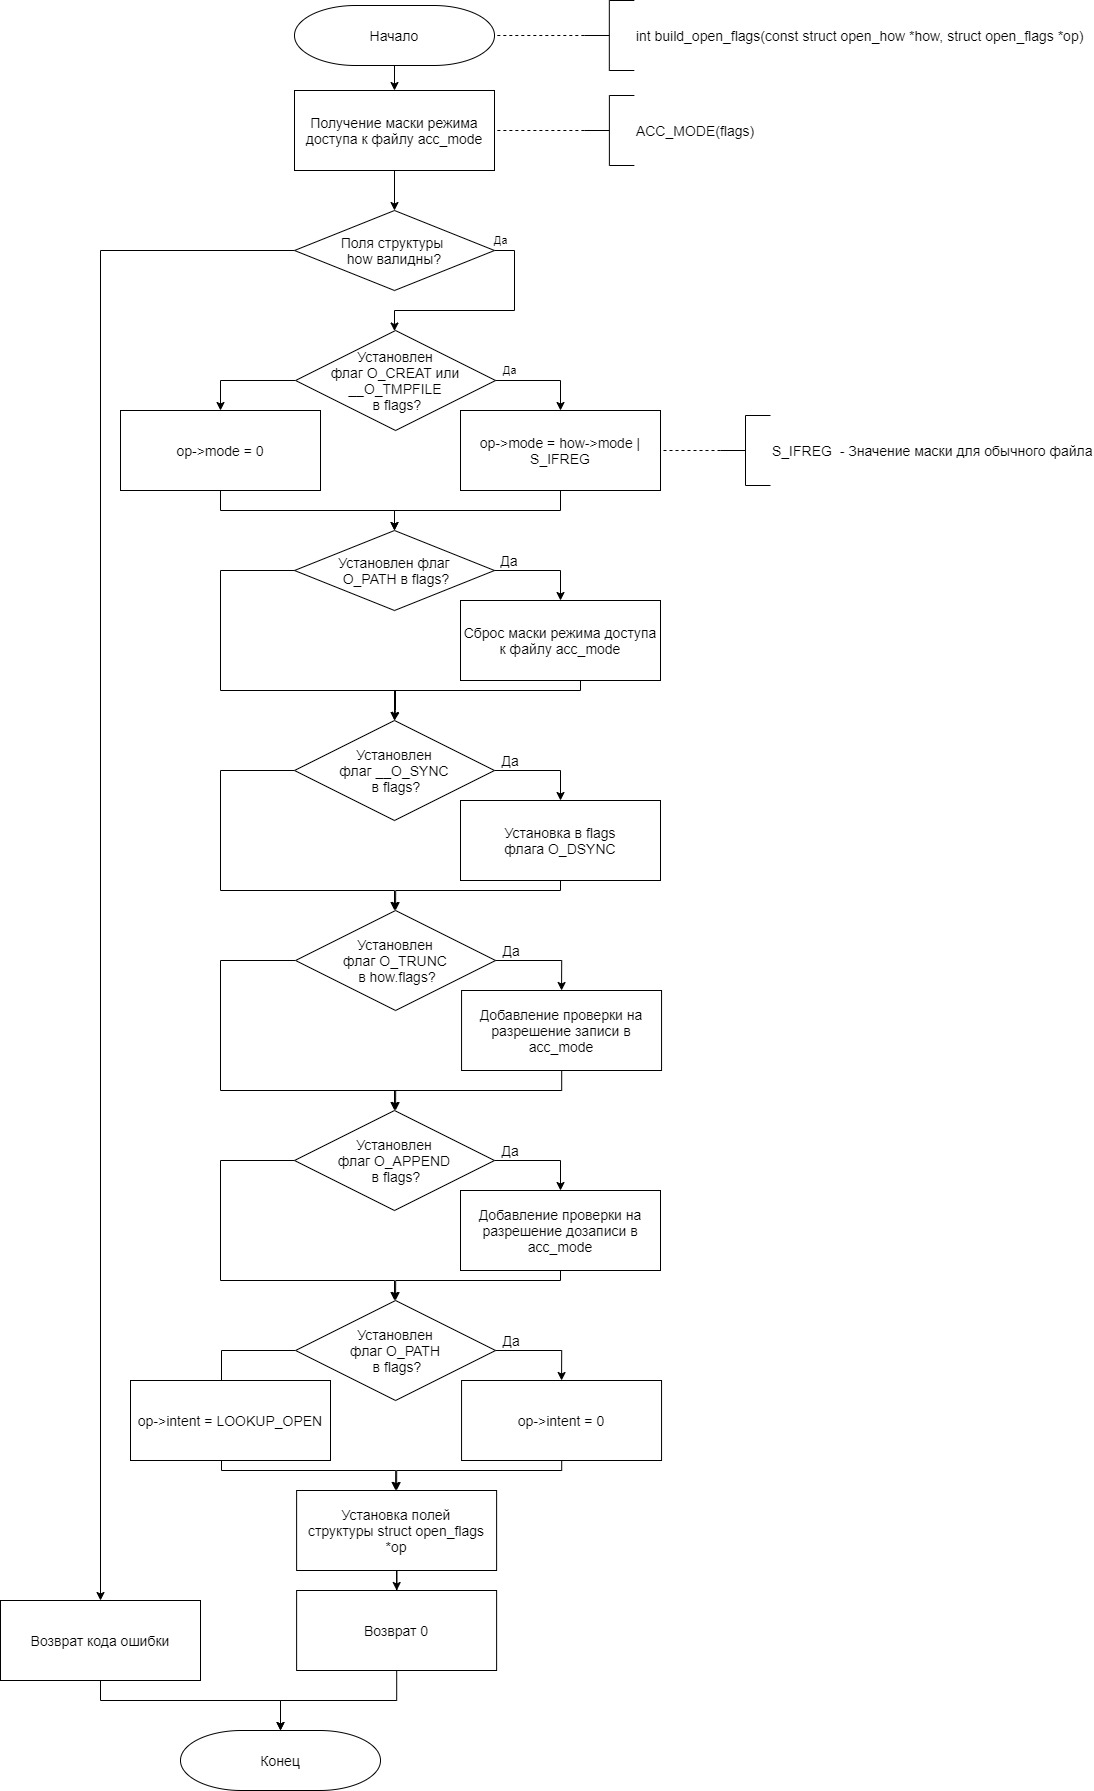
\includegraphics[scale=0.45]{img/build_open_flags.jpg}
\end{figure}




















\section{$\texttt{getname\_flags()}$}

\begin{figure}[H]
	\centering
	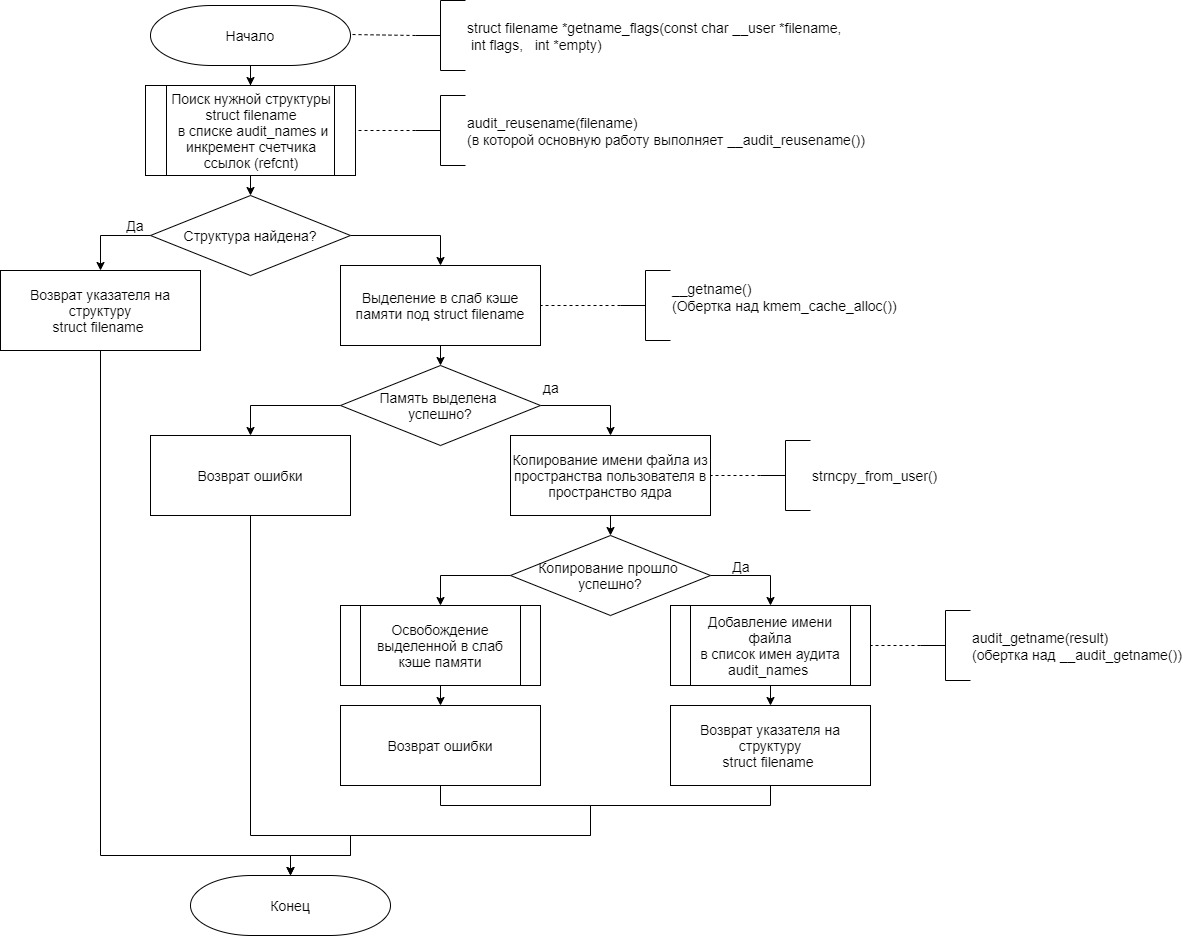
\includegraphics[scale=0.44]{img/getname_flags.jpg}
	%\caption{Схема структур программы №1}
	\label{fig:get_name_flags}
\end{figure}






\section{$\texttt{\_\_alloc\_fd}$}

\begin{figure}[H]
	\centering
	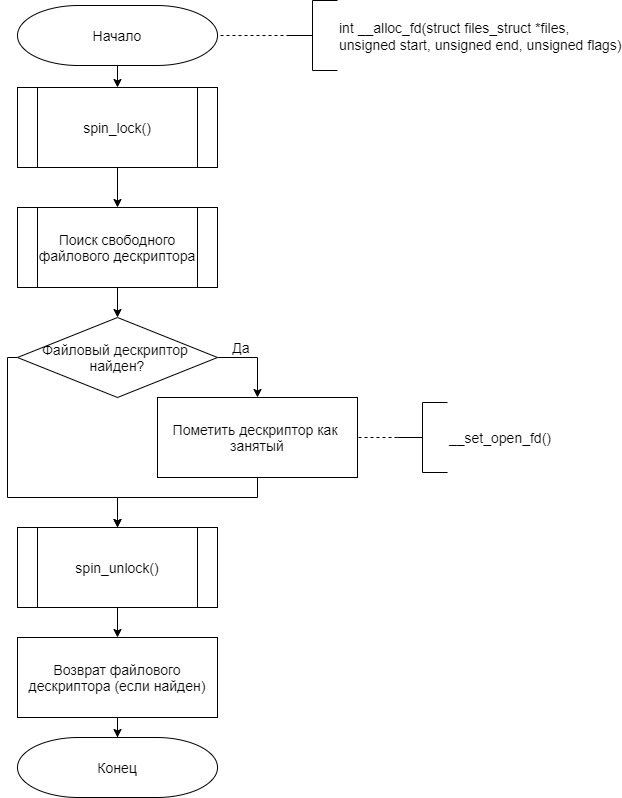
\includegraphics[scale=0.6]{img/alloc_fd.jpg}
	%\caption{Схема структур программы №1}
	\label{fig:alloc_fd}
\end{figure}













\section{$\texttt{do\_filp\_open}$}

\begin{figure}[H]
	\centering
	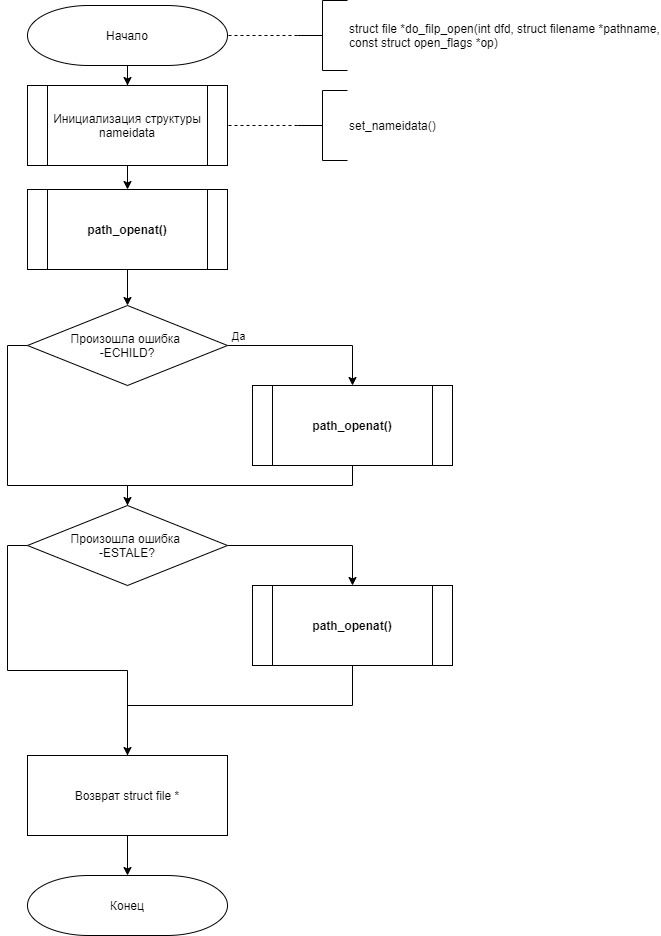
\includegraphics[scale=0.45]{img/do_filp_open.jpg}
	%\caption{Схема структур программы №1}
	\label{fig:do_filp_open}
\end{figure}




\section{$\texttt{path\_openat}$}

\begin{figure}[H]
	\centering
	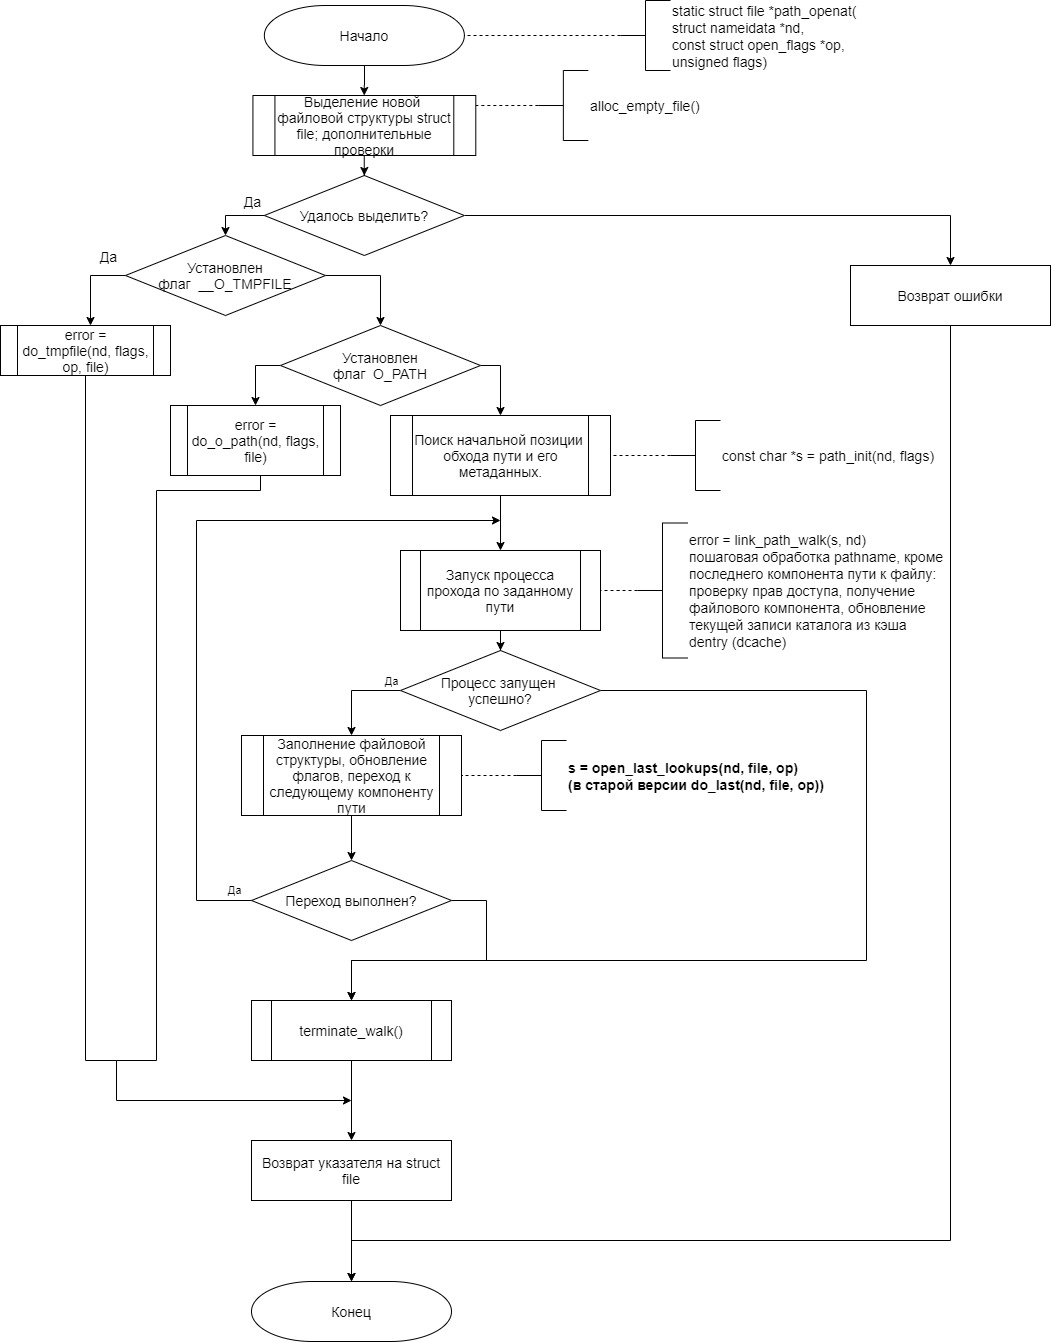
\includegraphics[scale=0.39]{img/path_openat.jpg}
	%\caption{Схема структур программы №1}
	\label{fig:path_openat}
\end{figure}



\section{$\texttt{lookup\_open}$}

\begin{figure}[H]
	\centering
	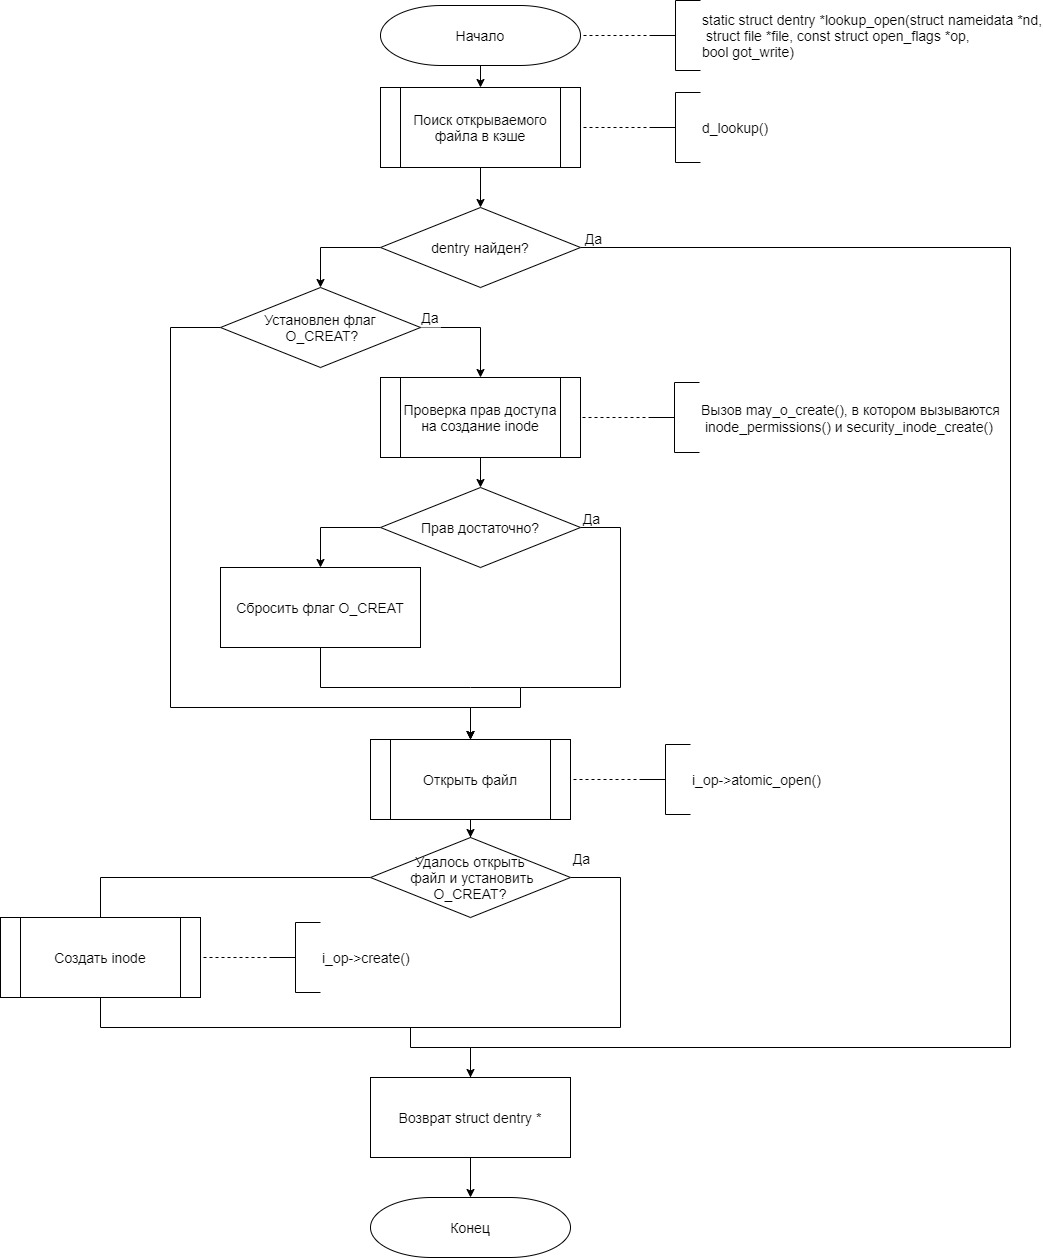
\includegraphics[scale=0.45]{img/lookup_open.jpg}
	%\caption{Схема структур программы №1}
	\label{fig:lookup_open}
\end{figure}

















% \section{Схема работы алгоритма функции $\texttt{build\_open\_flags}$}

%\begin{figure}[H]
%	\centering
%	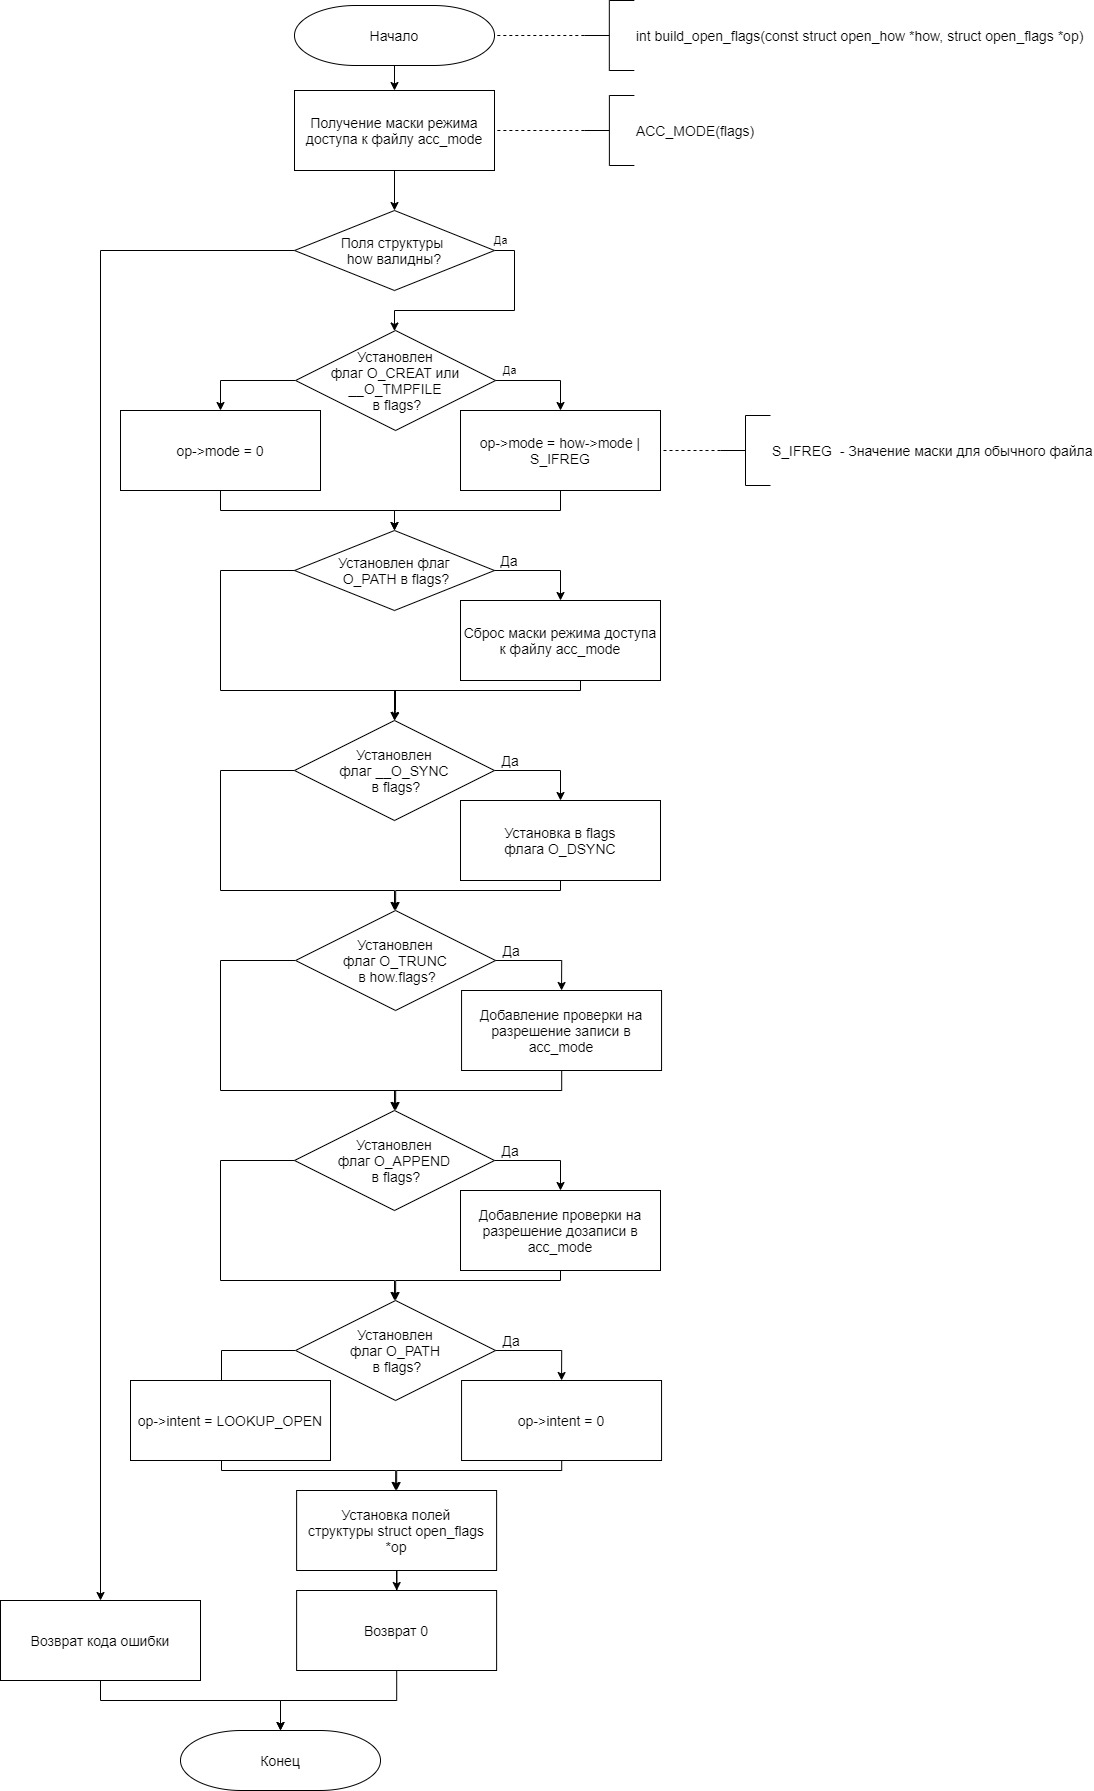
\includegraphics[scale=0.5]{img/build_open_flags.jpg}
%\end{figure}




\bibliographystyle{utf8gost705u}  % стилевой файл для оформления по ГОСТу
\bibliography{51-biblio}          % имя библиографической базы (bib-файла)
	
\end{document}
